\documentclass[a4paper,12pt]{report}
\usepackage{fontenc}
\usepackage[utf8]{inputenc}
\usepackage[english]{babel}
\usepackage[pdftex]{graphicx} 
\usepackage{listings}
\graphicspath {{figures/}}

\textwidth 6.3 in % Width of text line.
    \textheight 9.2 in
    \oddsidemargin 0 in      %   Left margin on odd-numbered pages.
    \evensidemargin 0 in      %   Left margin on even-numbered pages.
    \topmargin 0.2 in
    \headheight 0 in       %   Width of marginal notes.
    \headsep 0 in
    \topskip 0 in

\title{DRescue - Natural Disaster Alert and Rescue}
\author{Samantha Bandini\\Elisa Casadio\\Martina Giovanelli\\Anna Giulia Leoni\\Sofia Rosetti}
\date{\today}

\begin{document}

\maketitle

\tableofcontents

\chapter{Introduction}

The project consists in a monitoring and rescue system in case of natural disasters. 

There is a smartphone application which allows users to alert in the event of hearthquake, landslide, fire and other emergencies.
Alerts are collected and processed with the aim of informing the civil protection of the area in order to coordinate rescue teams.
Civil protection desktop applications communicate with each other to get information about available or occupied rescue teams.

User side there is a native Android application used to warn a natural disaster, sending an alert containing the position to the server.

Civil protection side there is a desktop application used to coordinate rescues.

Each civil protection manages a single district, but each rescue team can join different civil protections. This is why coordination is important in order to know real-time which teams are available and, if not, when they will be.


\chapter{Software development process}

(modalità di divisione in itinere dei task, meeting/interazioni pianificate, modalità di revisione in itinere dei task, scelta degli strumenti di test/build/continuous integration)\\
•	uno studente (ad esempio, chi ha l'idea del progetto) fungerà da product owner, oltre che da sviluppatore\\
•	in un meeting iniziale si rediga un product backlog, e si definisca un primo sprint organizzativo (preparazione della build, identificazione requisiti base e architettura)\\
•	si definiscano via-via delle sprint da 25-30 ore di lavoro (una settimana full-time), in modo da realizzarne 3-4 in tutto\\
•	si cerchi ad ogni sprint di ottenere risultati "tangibili", con già un valore per gli stakeholder (i docenti)\\
•	si tenga anche uno sprint backlog, e si facciano meeting frequenti, e meeting a inizio/fine sprint (con brevissimo report del risultato, anch'esso da tenere in versione)\\

*) Le scelte tecnologiche non dovrebbero essere anticipate troppo per ovvi motivi.. prima le fate prima impattano tutta la parte successiva e quindi diventano più difficilmente riconsiderabili (comunque in linea di principio ogni scelta potrebbero stare ovunque, dai requirement fino all'implementazione) \\



\section{Development methodology}
Agile

La gestione delle sprint si è svolta in modo flessibile a causa di impegni personali dei componenti.

%TODO da riguardare
Each Sprint started with the product backlog (where all the main tasks are defined) followed by the Sprint Backlog where all the created tasks were well discussed and divided in more defined and detailed subtasks. During the first 3-4 Sprints each member of the team used to volunteer to be assigned to one or more tasks. As the development continued, each member was assigned to a well defined and specified sub-system, creating a better organized environment where everybody knew exactly what the other was working on. At the end of each week, we used one hour of our time (Sprint Retrospective) to discuss about what went good and what had to be improved during the next Sprint

\section{Development tools}
Following development support tools have been used:

\begin{itemize}
\item \textbf{IntelliJ IDEA} as integrated software environment
\item \textbf{Java} and \textbf{Scala} as programming languages
\item \textbf{JUnit} and \textbf{ScalaTest} as testing tools
\item \textbf{Git} as version control system
\item \textbf{GitHub} as version control repository
\item \textbf{Gradle} as build automation system
\item \textbf{Travis CI} as continuous integration service
\item \textbf{Trello} as web project management application
\item \textbf{TeamViewer} as team collaboration and working tool
\end{itemize}

%TODO Test: JUnit e ScalaTest da specificare nelle singole implementazioni

\chapter{Requirements}
(2-3 facciate)
Attenzione ai requirement non funzionali: 1) non siano troppo vaghi altrimenti sono inverificabili, e quindi praticamente inutili; 2) il sistema è distribuito, quindi è inevitable dire cosa vi aspettate in termindi di robustezza a cambiamenti/guasti (quali?, come?), e scalabilità

\section{Functional requirements}

According to agile methodologies in the first sprint we wrote user cases like ``As.. I want.. For..", which have highlighted these functional requirements:

\begin{itemize}
\item A not logged user has to register or login to access the platform.
\item A user needs to view last fifty alerts of his area, to see what happens nearby.
\item A user needs to send an alert to inform civil protection about a particular event.
\item A user needs to view his profile to check his register information.
\item A user needs to change his password to update it.
\item A user needs to confirm an alert (upvoting it) to increase the alert reliability.
\item A civil protection has to login to access the platform.
\item A civil protection needs to receive alerts of its area to coordinate the rescues.
\item A civil protection needs to visualize in action rescues to have a general view of rescues and occupied teams.
\item A civil protection needs to enroll a rescue team in to send it when needed.
\item A civil protection needs to receive notifications when a team is occupied in order to know which ones to send.
\item A civil protection needs to decide which team is the most appropriate to send (at discretion of the civil protection user).
\item A civil protection needs to notify the sending of a team for a specific alert in order to intervene in case of emergency.
\item A civil protection needs to notify the end of a rescue to inform other civil protections that the team is available again.
\item The server has to forward the alerts and the upvotes to the civil protection of the area in order to warn it.
\item The server has to interact with the database as for user and civil protection requests in order to save datas.
\end{itemize}

\section{Non-functional requirements}
- Gli alert devono avere una certa "affidabilità", così da non "disturbare" la protezione civile con alert non veritieri o riempire il db con molte segnalazioni relative allo stesso evento (per questo utilizzati upvotes all'interno di alert)\\
In questo modo l'utente fa prima ad effettuare una segnalazione\\
Sul DB si ha una tabella con meno record e che quindi facilita l'esecuzione delle query\\
Lato protezione civile si vedono in cima alla lista gli ultimi alert e gli alert con upvote recenti\\
- App mobile user-friendly\\
- Aggiornamento real-time della view della protezione civile per alert-upvotes senza effettuare richieste specifiche.\\
- Mantenere le informazioni relative agli alert memorizzate su un DB

\chapter{Architectural design}

(pattern architetturali usati, componenti del sistema distribuito, scelte tecnologiche cruciali ai fini architetturali -- corredato da pochi ma efficaci diagrammi)\\

*) Ricordate che una scelta architetturale può ritenersi giustificata o meno (e dovremo capirlo) solo a fronte dei requirement che avete indicato\\

*) L'architettura deve spiegare quali sono i sotto-componenti del sistema (da 3 a 10, diciamo), ognuno cosa fa, chi parla con chi e per dirsi cosa -- i diagrammi aiutano\\

Disegnigno introduttivo

\section{Server-DB}
AWS: deciso in remoto per evitare di avere copie duplicate e necessità di ricreare DB e server

MySQL: deciso per compatibilità con le varie componenti utilizzate (più conosciuto/più documentazione), gratuito.
Indecise con no sql poi scelto mysql perché db parecchio grande e per avere sicurezze di non incorrere in spese.

\section{MVC Architecture}
The MVC design pattern decouples these major components allowing for efficient code reuse and parallel development.
%https://en.wikipedia.org/wiki/Model%E2%80%93view%E2%80%93controller

Con MVC si è gestito il modulo civilprotection in quanto è un applicativo desktop che comprende anche una parte rilevante di visualizzazione grafica.\\
E' stato necessario effettuare una gestione orientata alla gestione dei dati relativi alla protezione civile che sta utilizzando l'applicativo.\\
Disegno (controller grande + piccoli)\\
Il design MVC è stato gestito come in figura X.\\
Ognuna delle 4 view è associata ad un controller minore, il quale ha il riferimento ad un controller principale che ha il compito di interagire col modello.


\section{Data Access Object}
Data Access Object (DAO) is a commonly used pattern to persist domain objects into a database. The most common form of a DAO pattern is a class that contains CRUD methods for a particular domain entity type.
The pattern has these advantages:
\begin{itemize}
\item It separates the domain logic that use it from any particular persistence mechanism or APIs.
\item The interface methods signature are independent of the content of the implementation class. When you add a field to the Object of DAO, you don’t need to change the interface nor its callers.
\end{itemize}

A better pattern is Repository, it uses a metaphor of a Collection. This metaphor gives the pattern a tight contract and make it easier to understand.\\
In addition in this case, inheritance, abstract classes, and template methods are used to avoid duplicate code since all models need some common methods, this will be discussed in the next chapter.
So we have a GenericDAO, with the basic methods, from which all other DAOs extends.
In the following code segment is shown the GenericDao with methods insert, delete, selectByIdentifier and insertAndGet.\\
\begin{lstlisting}
public interface GenericDao {

    void insert(ObjectModel objectModel) 
    	throws DBDuplicatedRecordException, DBQueryException;

    void delete(ObjectModel objectModel) 
    	throws DBNotFoundRecordException, DBQueryException;

    ObjectModel selectByIdentifier(ObjectModel objectModel);

    ObjectModel insertAndGet(ObjectModel objectModel)
            throws DBQueryException, 
            		DBDuplicatedRecordException, 
            		DBNotFoundRecordException;
}

\end{lstlisting}

The \textit{insert} and \textit{delete} methods look identical to the methods of the simple DAO's, but the \textit{selectByIdentifier} method differs to the standard DAO’s \textit{findById} method by taking an ObjectModel object rather than the object identifier. 
Making this change you avoid to expose the type of ObjectModel identity to the interface.

In our case Repository pattern is realized with DAO.
\section{RabbitMQ MOM}
\subsection{Client-Server}
\subsection{Peer-To-Peer}

\chapter{Detail design}
%TODO
(pattern di progettazione, organizzazione del codice -- corredato da pochi ma efficaci diagrammi)\\
*) Il design di dettaglio "esplode" (dettaglia) l'architettura, ma viene concettualmente prima dell'implementazione, quindi non metteteci diagrammi ultra-dettagliati estratti dal codice, quelli vanno nella parte di implementazione

\section{Graphical User Interface Design}
\subsection{Mobile App}
\subsection{Civil Protection}

\section{Code organization}
Tutto all'interno dello stesso progetto dividendolo in moduli
Screenshot + descrizione moduli
\begin{itemize}
\item civilprotection
\item mobileuser
\item server
\item utils
\item utils-java
\end{itemize}

\section{Patterns}
\begin{itemize}
\item Builder: utilizzato quando si hanno più di 2/3 parametri
\item Template Method: utilizzato per la gestione delle risposte dal server e per raggruppare oggetti simili con metodi in comune per accedere ad oggetti nel database
\item Singleton: utilizzato per il coordinator
\item View-Holder: utilizzato per gli adapter Android
\item Static factory: utilizzato per la creazione della connessione al database
\item Factory pattern: utilizzato per recuperare i dao delle relative tabelle del database
\item Observer: utilizzato per gestire l'aggiornamento delle view a seguito di cambiamenti del model
\end{itemize}

\section{Communication messages}
Diagrammi di sequenza per RPC e forward + comunicazione tra CP
3 tabelle (mobile, alert, civilprotection)

Mobile user - server communication:

\begin{center}
\begin{tabular}{ |p{4cm}|p{4cm}|p{4cm}|p{2cm}| } 
\hline
Service 			& Request message 	& Response message		& Type 	\\
\hline
Sign Up  			& SignUpMessage(name, surname,email,pass word,phoneNumber)		& SuccessfulMessage 	& RPC	\\ 
Login 				& LoginMessage(email, password) 	& ResponseLoginMessage (UserImpl,List$<$Event TypeImpl$>$)	& RPC	\\ 
Request profile 	& RequestProfileMessage (email)		& ProfileMessage(User Impl)	& RPC	\\ 
Change password		& ChangePasswordMess age(email,oldPassword, newPassword)	& SuccessfulMessage	& RPC	\\
Get alerts		& RequestAlertsMessage (latitude,longitude)	& AlertsMessage(List $<$AlertsImpl$>$)	& RPC	\\
New alert		& NewAlertMessage(user ID,eventType,latitude, longitude)	& no response but ForwardObjectMessage (List$<$String$>$,Object Model)	& p/s	\\
Upvote alert		& RequestUpvoteAlert Message(userID, alertID)	& no response but ForwardObjectMessage (List$<$String$>$,Object Model)	& p/s	\\
\hline
\end{tabular}
\end{center}

Civil protection - server communication:

\begin{center}
\begin{tabular}{ |p{4cm}|p{4cm}|p{4cm}|p{2cm}| } 
\hline
Service 			& Request message 	& Response message		& Type 	\\
\hline
Login	& CpLoginMessage(cpID, password)	& RescueTeamsMessage (List$<$RescueTeamImpl$>$) 	& RPC	\\ 
Get alerts CP	& RequestCpAlertsMes sage(cpID,password)	& AlertsMessage (List$<$AlertImpl$>$) 	& RPC	\\ 
Register team at CP		& EnrollRescueTeamMess age(rescueTeamID,cpID)	& SuccessfulMessage & RPC	\\ 
Get CP of rescue team 	& GetAssociatedCpMess age(rescueTeamID)		& CivilProtectionsMess age(List$<$CivilProtec tionImpl$>$)	& RPC	\\ 
New team	& NewRescueTeamMess age(rescueTeamID,name, password,latitude,lon gitude,phoneNumber)	& SuccessfulMessage	& RPC	\\
Get not enrolled rescue teams & GetRescueTeamsNot EnrolledMessage	& RescueTeamsMessage (List$<$RescueTeamImpl$>$)	& RPC	\\
\hline
\end{tabular}
\end{center}

Civil protection - Civil protection communication:


\chapter{Implementation}

\section{Samantha Bandini}
In the DRescue project, Samantha Bandini contribution was mainly related to design and implementation of:
\begin{itemize}
\item Data Access Layer 
\item Handle Exception DB-Server in collaboration with Anna Giulia Leoni and Elisa Casadio
\item Handle MVC in civil protection in collaboration with Sofia Rosetti
\end{itemize}

\subsection{Data Access Layer}

Our application must access a database, so it needed some logic to handle database access. In order to keep the code clean and modular, the database access logic is isolated into a separate module, in our project is included in package\\ \texttt{server/src/main/java/it/unibo/drescue/database}. This package contains:\\

%TODO fix packages
\texttt{DBConnection.java} and \texttt{DBConnectionImpl.java}: Respectively the interface and the class used to model the access method to DB and its tables.\\
It uses two static factory method instead of constructor, this methods, \\ \texttt{getRemoteConnection()} and \texttt{getLocalConnection()}, are static methods that returns an instance of the class with some specific settings for environment, like address, username and password used to connect to DB. One advantage of this pattern is that in this way it has name, in this case it was useful for specifying the criteria to choose the connection (local or remote).\\
As specified in previous chapters the DAO pattern was used for Data Access Layer. Since the DBConnectionImpl class is the one that keeps the general information about the database, information about DB tables are also maintained here, like its relative DAO. Here is maintained the enum with all table's name and the method \texttt{GenericDaoAbstract getDAO(final Table table)} which is a factory that returns the Dao relative to that table.\\

And the packages:\\

\texttt{dao}: It contains all DAO with their interfaces as specified in detailed design chapter.\\
%TODO fix: add link
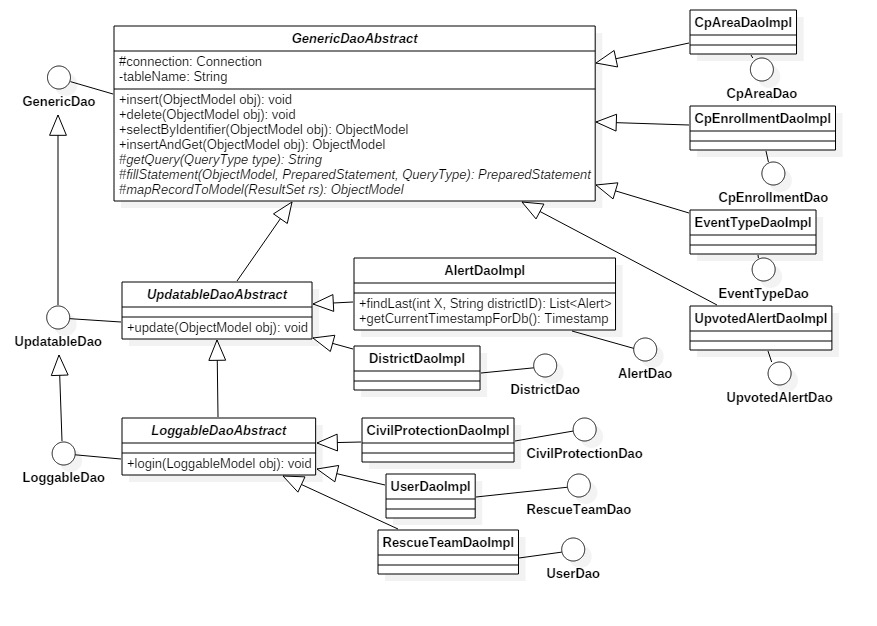
\includegraphics[width=\textwidth]{figures/ClassDiagram.jpg}
The DAOs are organized as specified in the partial class diagram above. Inheritance and template methods are used to group similar DAOs. The three main DAO's are GenericDao, LoggableDao, UpdatableDao. The GenericDao is the main class from which all others DAO extends, it contains the template methods insert, delete, selectByIdentifier, insertAndGet with abstract methods to be implemented in the classes that extend it.

The UpdatableDao contains the template method update, the LoggableDao contains the template method login and the abstract methods are:
\begin{itemize}
\item \texttt{String getQuery(final QueryType queryType)} Given a query type it returns the prepared query (a composed string) for this object
\item \texttt{PreparedStatement fillStatement(final ObjectModel objectModel, \\final PreparedStatement statement, final QueryType queryType)}: Given an object and a prepared statement it returns that prepared statement filled with the useful information to execute the specified query
\item \texttt{ObjectModel mapRecordToModel(ResultSet resultSet)} Get an object from a resultSet given, obtained from a select query by identifier
\end{itemize}

An example of a particular DAO is CpEnrollment, its method \\
\texttt{List<RescueTeam> findAllRescueTeamGivenACp(String cpID, boolean related)} has the parameter \textit{related} that is the criteria used to choose the query, since for the CpEnrollment we need both methods \texttt{findAllRescueTeamRelatedToACp} and \\
\texttt{findAllRescueTeamNotRelatedToACp}, with both returning a list of RescueTeam objects that differs only for the query. \\
%TODO check

\texttt{helper}: It contains the class DBInitializationStart used to initialize DB with static tables contents and some other data contained in externals file, to have something to start with.
The externals file are located in \textit{server/res}. The DBinitialization interface has a method used to insert into DB all objects listed in a json file, with a parameter \textit{table} that indicates the criteria, so in which table it has to be inserted, and the \textit{pathFile} that indicates the path where the file with objects is located.

To initialize the DB in this way, it was created in utils-java module, in package \texttt{src/main/java/it/unibo/drescue/database} a class \texttt{JsonFileUtils.java} with the generic method \texttt{<T> List<T> getListFromJsonFile(final String path, \\final Class<T[]> type)} that get a generic list of objects from a json file indicating the path of the file and the type of the class of the object to get.

\subsubsection{Travis configuration for mysql}
Tests that cover the database part must be run locally, so that they do not act on the remote database that is being used by the real application, but on a copy of this in local environment.
To do this, we had to prepare a .sql document to initialize all db tables and each of us, on a machine where SQL Server and SQL Workbench were installed, ran this file locally.
The problem came up when these tests had to be run in Travis. In addition to add the mysql service to the .travis.yml file, it was necessary to configure the credentials for Travis like in our local environment and also to create the DB with all tables. \\\
These rows has been added to .travis.yml file:\\
\texttt{before}\textunderscore\texttt{install:}\\
\texttt{- mysql -u root --password="" < travis.sql}
\\where travis.sql is a file .sql that contains all configuration specified above.

\section{Elisa Casadio}
The developed part mainly concerns the total or partial definition, design and development of the Android application and the server.

\subsection{Android application}
The code mentioned in this section is available in the \texttt{mobileuser} module.
\subsubsection{GPS}
GPS is a very important component within the application, as it is useful to indicate the exact location from which a user alert is sent and also to display all the alerts in the area where the user is located.

So, the application must have permissions to access the GPS, because the GPS is a sensitive data and it need to have the explicit consent of the user to be able to use it. Also, the device must have the GPS activated, because otherwise it would not be possible to understand where the user is and the latitude and longitude values could not be obtained.

The package \texttt{gps} contains an activity has been defined in which the required permissions and presence of the GPS provider are checked during creation and resume of activity. It also provides the latitude and longitude values, but if they aren't available it is setted a specific message. Using the \emph{observer} pattern, the activity is notified when the latitude and longitude values change or when the provider is disabled.

This activity is extended by all those activities that need to use the GPS, so that they can have the location values or check the provider.

\subsubsection{Layouts and Activities}
Four activities have been implemented with the relevant layouts to allow the user to send a new report, view the profile, change their password and the home page of application.

\begin{itemize}
\item \texttt{NewAlertActivity} in the package \texttt{alert} is the main feature that the application has, because it must allow the user to report a natural disaster. The class extends the GPS activity, because it needs to know the latitude and longitude values to show to the user and comunicate them to the server. In the layout, in addition to GPS values, it is given to user the possibility to select the type of natural disaster that occurs, by choosing between those in the database. The list of possible natural disasters is downloaded only whenever the user logs in so as not to slow down the operation and is saved between shared preferences of device.
\item \texttt{ProfileActivity} in the package \texttt{profile} shows the user data. The data are downloaded when the user logs in and they are saved in the shared preferences of the device. Each field is set by taking the value saved in the shared preferences that has a certain key. The keys that can be used are listed in the \texttt{PreferencesKey} enum in the package \texttt{utils}. From this activity is possible to reach the activity for change the profile password and do logout. The logout is very simple, just delete all the data saved in the shared preferences.
\item \texttt{ChangePasswordActivity} in the package \texttt{profile} allows the user to change his password. So, it is necessary to take the old and the new password, the user email and update his record on database. The layout shows three fields where the user can write. Each field must comply with two rules: the password must be at least 6 characters long and it must contain only alphanumeric characters.
\item \texttt{MainActivity} shows a RecyclerView where the CardView are arranged in a grid. Each CardView contains a title, an icon and a string with the class name that must start at the click of the CardView. The titles, the icons and the strings are listed in \texttt{arrays.xml} in \texttt{res} folder in the form of array. In order to handle the RecyclerView, it was need to use the \emph{Observer} pattern, the \emph{Adapter} pattern and the \emph{ViewHolder} pattern. Using the \emph{Observer} pattern, it was possible to notify when the user click on a specific CardView and to open the relative activity. The \emph{ViewHolder} pattern has allowed to set the correct fields of each CardView and the \emph{adapter} pattern has been the bridge between activity and the ViewHolder. \texttt{MainActivity}, during its creation or its resume, controls that the shared preferences are not empty. If this is not the case, it means that the user has logged out, so it need to go back to \texttt{SplashActivity} where the user can log in again.
\end{itemize}

\subsubsection{Connection between authentication and profile activities and server}
After performing all the layouts and basic activity operations, the connection between the activities and the server was added using the classes contained in the \texttt{connection} package.

The deployed connection is about authentication and profile activities. In all these cases, the type of communication is RPC, so all requests were made using \texttt{RabbitAsyncTask} class. The responses are \texttt{AbstractResponse}, so they were handled differently depending on what was needed to get. For more detailed explanation about \texttt{RabbitAsyncTask} and \texttt{AbstractResponse} see the dedicated section of developer Anna Giulia Leoni.

First, it was necessary to create a message to be sent to the server in order to forward the request, then check the presence of the Internet connection (both through mobile and Wi-Fi connecition). This check was essential because forwarding a request without connection could cause an application crash. Also, being necessary to recive a response from the server, it has entered a progress dialog that blocks the user's activity until the application receives any response from the server.

\begin{itemize}
\item \texttt{SignUpActivity} in package \texttt{authentication} was implemented by Anna Giulia Leoni and refactored by Elisa Casadio. The request message consists of all the data that the user has entered during the registration. The response message consists in a simple successful message, which confirm the database registration.
\item \texttt{LoginActivity} in package \texttt{authentication} has the request message assembled by the credentials of user. The response message consists in a message with the user data and a list of natural disaster. All this data are saved in shared preferences to use them in future in some requests or in the application. It has preferred to have all essential information at the user login, because it has avoided slowing down the user when displaying some views, such as profile or new alert.
\item \texttt{ChangePasswordActivity} in package \texttt{profile} has the request message assembled by the new and old password and the user email, the latter derived from shared preferences. The response message is a successful message, which confirm the update of password.
\end{itemize}

\subsubsection{Graphics}
To get a user-friendly application, the graphics were helpful. First, the basic colors that would have featured the application were choosen. Tones on green and yellow were chosen so that application could recall nature. Colors are listed within \texttt{colors.xml} so they can be used by all layouts. To have a minor repetition of the code, xml tags have been redefined within \texttt{styles.xml}, while \texttt{strings.xml} and \texttt{dimens.xml} have all the strings shown in the view and all the dimensions of the components used. Finally, the material icons were selected for use within the application.

\subsection{Server application}
\subsubsection{MobileuserService}

\section{Martina Giovanelli}
\section{Anna Giulia Leoni}

The developed part mainly concerns the development of the Server application and the Android one, but also  a little part in the Civil Protection application.

\subsection{Server application}

All the code referred into this section is located into module \texttt{server/scala}.

\subsubsection{Service response, Service forward}
In order to handle the sending of a response and the forward of a message server side, \texttt{ServiceResponse} and \texttt{ServiceForward} traits were created in package \texttt{connection}. These traits extend \texttt{ServiceOperation} overriding and implementing in different ways \textit{handleDBresult}. 

Services that can handle both response and forward extends \texttt{ServiceResponseOr\\Forward} trait which extends both \texttt{ServiceResponse} and \texttt{ServiceForward}. This was possibile because Scala allows implementing functions in traits and multiple inheritance on traits. Basing on the content of the \textit{properties} parameter that came together with the message through RabbitMQ, it is discriminated if the message has to be forwarded or needs a reply and the appropriate \textit{super} method is called.
\\More specifically if the \textit{properties.getReplyTo} content is a valid string then represents the name of the queue to which send the response message returned from \textit{accessDB} method. Otherwise the result of the \textit{accessDB} method is a \texttt{FrowardObjectMessage} containing the ObjectModel to forward and the queues name to which forward it.
\\This behaviour is tested using inside \texttt{TestClientServerCommunication} class in \texttt{test} folder of package \texttt{connection}.
\\
%TODO diamond inheritance pic?

\subsubsection{AlertsService}
Case class \texttt{AlertsService} in package \texttt{connection} extends \texttt{ServiceResponseOrForward} and manages messages requests related to alerts both from mobileuser and civil protection. More specifically these messages are shown in the detail design section.

In handling new alerts and upvotes messages is also necessary to retrieve the civil protections related to the zone from which the alert was sent to forward the alert or the upvote to the rights civil protections. Furthermore in handling new alerts and requests of alerts from mobile, methods of the Geocoding class were used to calculate the district to which register the new alert or to which get the alerts.

\subsection{Android application}

All the code referred into this section is located into module \texttt{mobileuser}.

\subsubsection{Layouts and Activities}
\texttt{ToolbarActivity} is extended by all the activities of the app. As the docs says the native ActionBar behaves differently depending on the Android version the device is using, we used Toolbar instead of ActionBar which has a more uniform behaviour.

Activities have been implemented with the related layouts to allow the user to sign up, login, get and upvote alerts.
\begin{itemize}
\item \texttt{SplashActivity} represents the splash screen of the app where the user can select to sign up or login
\item \texttt{SignUpActivity} and \texttt{LoginActivity} in package \texttt{authentication} represent respectivly the activity that contains the fields that the user must fill to sign up and login. Some checks are made on the validity of the email address and the match between password and confirm password at sign up.
\item \texttt{UpvoteAlertActivity} in package \texttt{alert} represents the activity that contains a list of existing alerts that the user can upvote to increase their reliability. It extends \texttt{GpsActivityImpl} because latitude and longitude of the user are needed to correctly download alerts of its district. \\
The alert list is presented within the app using Adapter and ListView. The \texttt{Alert Adapter} allows access to data and creates the corresponding view based on the layout provided for each alert of the given list. Inside the Adapter the ViewHolder pattern has been used to limit the number of calls to \textit{findViewbyId} method. This ways, this methods is invoked once for every items of the list passed at constructor and references to layout elements are stored in an \texttt{AlertViewHolder} instance associated with convertView with \textit{View.setTag} to be used for next items.
\end{itemize}

%TODO digramma classi?

\subsubsection{Connection to server}
The package \texttt{connection} contains the classes used to communicate to the server and eventually parse the response.
\\To achieve this goal, Android AsynkTask were used. AsynkTask allows to perform background operations and publish results on the UI thread without having to manipulate threads and/or handlers. Within the \textit{doInBackground} method is contained the code to open the connection to the server, send the message and eventually waiting for a response.

More specifically two AsynkTask were created:
\begin{itemize}
 \item \texttt{RabbitAsyncTask} to perform RPC, returning a String result that represents the server response in json format. If the communication timeout is reached or in case of exception during the communication the result consists of an error. The received result is passed to an handler, represented by a class implementing the \texttt{RequestDelegate} interface, in our case \texttt{AbstractResponse} class, which deserializes it basing on message type and addresses it to the abstract methods \textit{onSuccessfulRequest} or \textit{onErrorRequest} implemented for each request to perform specific operations basing on it.
 \item \texttt{RabbitPublishAsyncTask} to send messages using the publish/subscribe paradigm, returning a boolean result that represents the sending outcome. The result is passed to an handler, represented by a class implementing the \texttt{PublisherDelegate} interface, which performs different operations basing on it.
\end{itemize}
The connection to the server was added into the activities of package \texttt{alert} using the above classes. Before sending the message to the server it is always checked that the device is connected to the netword and, if needed, if latitude and longitude values are correct. More specifically
\begin{itemize}
 \item in \texttt{NewAlertActivity} a \texttt{NewAlertMessage} containing the alert data is created, sent and the result of the sending is shown to the user.
 \item in \texttt{UpvoteAlertActivity} a \texttt{RequestUpvoteAlertMessage} containing the upvote data is created, sent and the result is shows as above; a \texttt{RequestAlertsMessage} containing user position is sent through RPC and on receiving the alert list of his district the adapter must be notified. If timeout is reached or an error occurr an error message is shown.
 
\end{itemize}

\subsection{Civil Protection application}

\subsubsection{RescueTeamConsumer}
%TODO

\section{Sofia Rosetti}
In the DRescue project, Sofia Rosetti contribution was mainly related to design and implementation of:

\begin{itemize}
\item Geocoding and reverse geocoding management
\item Model interfaces and classes
\item Civil protection views
\item Civil protection Model-View-Controller
\end{itemize}

\subsection{Geocoding and reverse geocoding management}
The geocoding and reverse geocoding service needed inside the project were designed and implemented using the Google Maps Geocoding API.

As Google explains, geocoding is the process of converting addresses (like a street address) into geographic coordinates (like latitude and longitude), while reverse geocoding is the process of converting geographic coordinates into a human-readable address.

As for the requirements of the project, it has been necessary to retrieve latitude and longitude coordinates giving a String corresponding to a generic address. This has been possible thanks to a \textbf{geocoding} request. The relative response consists in a JSON containing two root elements, ``status'' and ``results''. The ``results'' element contains an array of geocoded address and geometry information. From the geometry information it has been possible to retrieve the location, which returns latitude and longitude coordinates. 

Instead, \textbf{reverse geocoding} requests have been used to retrieve a district acronym (e.g. FC, RA, RN...) from latitude and longitude coordinates. The relative response contains a ``result'' element here too: instead of the geometry information, in this case we needed the ``address\_components'' information. 

It is composed of different elements like ``country'', ``root'' or ``street\_number'', but the interested one was ``\texttt{administrative\_area\_level\_2}'', which has a short name corresponding exactly to the district acronym we needed.

The \texttt{utils/src/main/java/it/unibo/drescue/geocoding} package contains geocoding interface, relative implementation class and exception class. Geocoding interface provides only two methods \emph{getDistrict()} and \emph{getLatLng()} that meet exactly the two requirements described above.

The \texttt{utils/src/test/java/it/unibo/drescue/geocoding} package contains a JUnit class test which verifies a proper operation.

\subsection{Model interfaces and classes}
In package \texttt{utils-java/src/main/java/it/unibo/drescue/model} there are all model interfaces and classes.

Every model entity represents one database table with all its attributes, so every interface provides methods to access and set the corresponding fields.

In the same package some other classes ending by ``Builder'' can be found. This because for class constructors with more than three fields the Builder pattern has been used.

Every model class has been tested writing JUnit test classes, which can be found under the \texttt{utils-java/src/test/java/it/unibo/drescue/model} package.

\subsection{Civil protection views}
In order to mantain most of civil protection module implemented using the Scala language, views have been created by hand with \textbf{ScalaFX}. 

Views have been organized as following.

There is a \texttt{MainView} scala class, which represents the ``container'' class and has container elements, like \textit{stage} and \textit{scene}.
Then, four scala classes (\texttt{LoginGrid}, \texttt{HomeGrid}, \texttt{EnrollTeamGrid} and \texttt{ManageRescuesGrid}) represent the \textit{GridPane} which changes depending on the view to be displayed.
Every \textit{GridPane} is built with a row-column structure that allows to position elements and let them cover more than one row or one column.

The \texttt{MainView} provides a method to change the view that creates a new specific grid corresponding to one of the previous classes.

A \texttt{ViewConstants} object has been implemented too with the purpose of collecting all used constants and remove all magic numbers inside view classes.

\subsection{Civil protection Model-View-Controller}
Individual contribution in civil protection Model-View-Controller was firstly focused on the base arrangement of links between the views in consequence of all buttons pressure.

Every button has been provided of a mouse event able to catch the mouse click. So relative controller methods are called and all relative actions are performed.

Part of the individual contribution was then oriented to implement two scala classes that belong to the civil protection local model.
The \texttt{AlertEntry} and \texttt{EnrolledTeamInfo} classes have been created to simplify insertion and values retrieval from the \textit{TableView} elements contained in the relative views. An \texttt{AlertEntry} element represents a table entry of the \texttt{HomeGrid}, because it's necessary to show the alert ID, the timestamp, latitude and longitude, the user and the district ID, the event name and the upvotes with a table representation. Similarly, the an \texttt{EnrollTeamInfo} element represents a table entry of the \texttt{ManageRescuesGrid}, because in this case it's necessary to show the team ID, name and phone number, if the team is available or not, the ID of the civil protection which occupied the team and the ID of the alert for which the team has been sent.

These two classes are also used in the \texttt{CivilProtectionData} class, which represents the model that every civil protection needs to mantain locally in order to get last alerts list and to manage rescue teams.

\section{Common parts}
%TODO Common part
I messaggi sono stati implementati a seconda delle necessità facendo per ognuno i test.

\subsection{Samantha Bandini - Sofia Rosetti}

\subsubsection{MVC (focus home e login)}
Il codice è stato organizzato con una suddivisione in package (model vero in altro modulo, model locale in localmodel, controllers in controller e views in view).\\
E' stato definito il model da passare al controller principale (CivilProtectionData).\\
L'aggiornamento delle view è stato impostato utilizzando il pattern Observer. Ad ogni cambiamento del modello la relativa view viene notificata e attraverso un ObservableBuffer viene aggiornata.\\


\subsubsection{Model update management}
AlertConsumer (è un consumer di RabbitMQ che rimane in attesa su una coda per ricevere i messaggi di ForwardAlertMessage e ForwardUpvotedAlertMessage; quando arrivano provvede all'aggiornamento del model) e RequestHandler (serve per far partire una future che ritorna un risultato che è la risposta che deve essere interpretata dal controller in quanto è un messaggio codificato tramite formato JSON)






\subsection{Samantha Bandini - Elisa Casadio - Anna Giulia Leoni}
Eccezioni

\subsection{Elisa Casadio - Anna Giulia Leoni}
\subsubsection{Server structure}
The code executed on server is located inside the \texttt{connection} package in \texttt{server} module.

\begin{itemize}
\item \texttt{ServerMain} represents the main class of the module, contains the code to setup the connection to RabbitMQ broker and runs all the services.
\item \texttt{Service} is a case class that represents a generic service. A new channel is created on the given connection and a new \texttt{ServerConsumer} is added to the channel and consume on the given queue.
\item \texttt{ServerConsumer} is a simple server-side consumer extending the default RabbitMQ consumer and overriding the \emph{handleDelivery} method called when consuming a message. Furthermore, a class implementing \texttt{ServerOperation} trait must be passed to the consumer in order to access database and handle potentially the returning result. In case of \emph{accessDB} method throw an exception, the error is logged, otherwise the result is handled. 
\item \texttt{ServiceOperation} is a trait modelling a general service to access database and handle the result. This trais is implemented by all classes that represent the specific services. The \emph{accessDB} method is where concreate access is using the data access object.
\end{itemize}

\subsubsection{Server configuration}
Anna Giulia following AWS Guidelines setup a preconfigured instance with RabbitMQ called \emph{Bitnami}.

Elisa, however, configured the instance Linux machine. First, the Java 8 JDK and Scala 2.12.2 are installed to can run the application. A service is created so that the server application can always be active on the machine. The \texttt{drescue-server.sh} bash file, containing the script to create, start and stop the service on the machine, is added to \texttt{/etc/init.d/} folder. Inside the script, there is the command to execute the application jar.

\subsection{Martina Giovanelli - Anna Giulia Leoni}

\subsubsection{Setup the connection}
The package \texttt{connection} inside \texttt{utils-java} module contains the classes used to setup the communication through rabbitMQ used in every other module that needs to communicate with the server or other clients.
\\\texttt{RabbitMQConnectionImpl} class implements \texttt{RabbitMQConnection} interface and contains methods to setup, close and get the real TCP connection with the RabbitMQ broker by setting the host address, port, username and password. 
\\\texttt{RabbitMQImpl} class implements \texttt{RabbitMQ} interface and contains methods to setup, get and performs other operations related to the virtual connection (\textit{channel}) created on the TCP one like sending a message or adding a new consumer on the channel consuming on a specific queue.

Definizione struttura messaggi (message solo per comunicazione punto-punto e abstract message per routing)

Select in enrollcontroller

%TODO chapter or section?
%\chapter{Testing}

\chapter{Retrospective}

(descrizione finale dettagliata dell'andamento dello sviluppo, del backlog, delle iterazioni; commenti finali)\\

*) Cercate di dare una idea di quanto pensate che i vostri test automatizzati coprano il codice e dove: è importante per stimare il potenziale impatto di una modifica al software\\


Si noti che la retrospettiva è l'unica sezione che può citare aneddoti di cosa è successo in itinere, mentre le altre sezioni fotografano il risultato finale. Se gli studenti decideranno (come auspicato) di utilizzare un product backlog e/o dei backlog delle varie iterazioni/sprint, è opportuno che questi siano file testuali tenuti in versione in una cartella "process", così che sia ri-verificabile a posteriori la storia del progetto.

%TODO riassumere e preparare i file per il repository (process/sprints/report)
1 Sprint
Organizzazione per capire un po’ le competenze di ognuna.

Suddivisione generale compiti 

Decisione di come tenerci aggiornate (tools)

Molti documenti su google drive (su cui lavorare in contemporanea)

Alcuni file su dropbox (apk o file utili per configurazioni al pc)

Product backlog (difficoltà stima tempi)

Diagrammi di sequenza 

Schemi su excel per messaggi da preparare per le varie code

Configurazione degli ambienti

2 Sprint 

Inizio configurazioni di base (orientate su server e db) 


-	Fatte prove per impostare la macchina per capire se potesse essere quello che poteva servire a noi (nessuna di noi aveva mai utilizzato aws o configurato una qualsiasi macchina linux con questo scopo prima)
-	Abbiamo molti dati e per essere sicure di avere un sistema aggiornato e persistente almeno per quanto riguarda alert e protezioni civili, si è ritenuto importante mantenere memorizzate alcune informazioni e “predisporre” il db per futuri cambiamenti, aggiornamenti

\section{Encountered issues}
Scelta AWS dopo perdita di tempo con Google App Engine

Incompatibilità Scala-Android

Pessimo supporto di IntelliJ con più moduli tra cui Android (Android ILogger)

Il DB poteva esser fatto in Scala ma la valutazione è stata fatta troppo tardi.

I DAO comportano duplicazione di codice. Si è cercato di gestire questo aspetto il meglio possibile.

Per consegnare entro i 2 mesi dall'accettazione del progetto l'ultima parte (civilprotection) è stata implementata senza eccellenza tecnica: questo per completare i principali requirements inizialmente definiti.

Difficoltà nella stima delle tempistiche.

\section{Final judgement}

\section{Future developments}
Fornire indicazioni alla protezione civile per aiutare nella scelta di un soccorso (già gestito lato DB-server): Rilevanza per alert con molti upvote / in base alla popolazione della zona, Algoritmo intelligente per la selezione della squadra in base alla distanza

CP: Mappa e possibilità di filtrare sui tipi di eventi

Zone di intervento delle CP che possono essere intersecate (già gestito lato DB-server)

App per le squadre di soccorso e per i soccorritori

Eventi realmente accaduti e relative statistiche

Estensione dell'applicazione mobile per altre piattaforme + miglioramenti (modifica profilo utente)

Live rescues: necessita salvataggio soccorsi su DB (evento accaduto, CP che ha fatto partire il soccorso e squadra di soccorso)

Sicurezza lato protezione civile per login (si è pensato con token/autenticazione)

User stories in grigio

\end{document}


















\newpage

Some useful latex commands:\\

\begin{itemize}
\item FirstItem  \texttt{A command}\\


\item Something Big: what it does: \\
- \textit{Something}, what it does.\\
- \textit{Other}, what it does.

\end{itemize}

\section*{A section}

\subsubsection*{A subsection}
Something $"\texttt{some formatted code}:\textbf{code}"$\\

NOTE Something: $command$ (to write a method name for example) or use it for field name like $player\textbf{ID}$. 

\end{document}


    
    
